\section{The ScapeGoat framework\label{sec:approach}}
%\section{Adaptive optimistic monitoring with the ScapeGoat framework\label{sec:approach}}

%\todo{Completely change this section !!! We need to make the link with the background here, and to provide a picture with an overview}

Our optimistic adaptive monitoring system extends the Kevoree platform with the following principles: i) component contracts that define per-component resource usage, ii) localized and just-in-time injection and activation of monitoring probes, iii) heuristic-guided faulty component detection. The following subsections present an overview of these three principles in action. 
%The monitored system follows the principles of component based software engineering.
%Each component is augmented with a contract that defines their expected resource usage.
%The contract specifies how the component is supposed to use, for example, memory, I/O and CPU resources.
 
%  \item \textbf{Localized and just-in-time injection and activation of monitoring probes.}
%Under normal conditions, our monitoring system performs lightweight global monitoring of the application.
%When a problem is detected at the global level, we activate local monitoring probes on components.
%Probes are synthesized according to the components' contracts to limit \hl{[capacity and?]} overhead.
%Thus, fine-grain monitoring is only applied when needed and only on the resource-data of interest.

% \item \textbf{Heuristic guided search of the problem source.} 
%To reduce latency and maintain an acceptable overhead, we use a heuristic to guess the locality of the faulty components.
%This heuristic is used to select where we inject and activate our monitoring probes.
%In short, it calculates suspected components.
%Our heuristic leverage the use of models@run.time by assigning a greater probability to recently updated components 
%\end{itemize}


\subsection{Specifying component contracts} \label{componentcontract}
%\assignedtodo{Inti}{Improve the contract as reviewer 3 suggested. (more relevant if using patterns based on the evolution of %values rather than maximum values)}

In both the Kevoree and ScapeGoat approaches, we follow the contract-aware component classification~\cite{Beugnard:1999:MCC:619042.621275}, which applies B. Meyer's Design-by-Contract principles~\cite{Meyer:1992:ADC:618974.619797} to components.
%This framework proposes to apply B. Meyer's Design by Contract~\cite{Meyer:1992:ADC:618974.619797} principles to components with an attempt at generalization.
%ScapeGoat mainly introduces the fourth level of contract (\textit{Quality of Service}) in Kevoree in supporting the specification of instant worst case situation for memory consumption, CPU and Input/Output resource consumption and time period average for the same resources kinds. 
In fact, ScapeGoat provides Kevoree with \textit{Quality of Service} contract extensions that specify the worst-case values of the resources the component uses.
The resources specified are memory, CPU, I/O and the time to service a request.
The exact semantic of a contract in ScapeGoat is: \textit{the component will consume at most $X$ resource if it receives at most $N$ requests on its provided ports.}  
%The resources specified are memory, CPU, I/O and request throughput.  

For example, for a simple Web server component we can define a contract on the number of instructions per second it may execute \cite{Binder200645} and the maximum amount of memory it can consume.
The number of messages can be specified per component or per component-port.
In this way, the information can be used to tune the usage of the component roughly or detailedly.
An example is shown in Listing~\ref{contractspec}.\footnote{Contract examples for the architecture presented in section~\ref{sec:motivatingexample} can be found at \url{http://goo.gl/uCZ2Mv}.} This contract extension follows the component interface principle~\cite{Henzinger03}, and allows us to detect if the problem comes from the component implementation or from a component interaction.
That is, we can distinguish between a component that is using excessive resources because it is faulty, or because other components are calling it excessively.


\lstset{frame=tb,
  aboveskip=3mm,
  belowskip=3mm,
  showstringspaces=false,
  columns=flexible,
  basicstyle=\color{black}\scriptsize,
  numbers=none,
  numberstyle=\color{gray}\scriptsize,
  keywordstyle=\color{blue}\scriptsize,
  commentstyle=\color{dkgreen}\scriptsize,
  stringstyle=\color{purple}\scriptsize,
  breaklines=true,
  breakatwhitespace=true,
  tabsize=2,,
  captionpos=b,
  language=java
}

\begin{lstlisting}[escapeinside={(*}{*)},caption=Component contract specification example,label=contractspec,float=!h]
add node0.WsServer650 : WsServer

//Specify that this component can use 2580323 CPU 
//instructions per second
set WsServer650.cpu_wall_time = 2580323 intr/sec 

//Specify that this component can consume a maximum of 15000
//bytes of memory
set WsServer650.memory_max_size = 15000 bytes

//Specify that the contract is guaranteed under the assumption that 
//we do not receive more than 10k messages on the component and 
//10k messages on the port named service
//(this component has only one port)
set WsServer650.throughput_all_ports = 10000 msg/sec
set WsServer650.throughput_ports.service = 10000 msg/sec

\end{lstlisting}

%They introduced a classification of contracts in four levels. 
%It can be summarized as:
%\begin{itemize}
%\item \textbf{Syntactic} (or basic) The goal is to make the system work. 
%It is generally specified with Interface Definition Languages (IDLs), as well as typed object-based or object-oriented languages.
%It ensures the components can be assembled.
%\item \textbf{Behavioral} The goal is to specify each operation. It is generally specified with a couple of assertions:
%a precondition and a postcondition. It ensures the operations offered and required are not only
%syntactically compatible but also semantically.
%\item \textbf{Synchronization} The goal is to specify the coordination of operations. It can be specified with an
%automaton labeled with operations. It ensures the operations are used in the proper order.
%\item \textbf{Quality of Service} The goal is to quantify a few features associated to operations. Performance, availability and quality of result can be specified and negotiated at that level.
%\end{itemize}

%Scapegoat approach is mainly built on top of Kevoree (section~\ref{sec:kevoree}). Kevoree supports only syntactic contracts between components. We introduce for Scapegoat a way \hl{to specify behavioural contracts, synchronization contract and quality of service contracts}\todo{Ok we propose something about "behavioural contracts with resource useage stuff but I'm not sure we propose something else...}. For synchronization and behavioral contract, we mainly reuse previous work~\cite{BaraisDuchien05} to provide a language for the specification of these contracts. To specify quality of services, Scapegoat introduces 
%
%As a basic example, a component \emph{A} can specify two ports with operations (level 1). 
%These operations can have pre and post conditions (level 2), the architect can provide a synchronization contract to specify that these ports cannot be accessed simultaneously (level 3) and that it can consume percent of CPU in a peak and an average of 10 percent of CPU resource per minute. \hl{SHOULD WE PROVIDE A REAL COMPONENT SPECIFICATION, SHOULD WE DISCUSS HOW WE infer these contract ?}
%\hl{(Johann) I think we should provide a real example here but not how we infered it}\todo{What are the levels ?}

\subsection{An adaptive monitoring framework within the container} \label{monitorContainer}

%In Scapegoat, the behavioral and synchronization contract correctness are not managed by the container.  To guarantee the behavioral component contracts, assertions are embedded at runtime within the component implementation, they can be activated on demand. In Kevoree, to guarantee concurrent access to ports, they are protected behind an actor model~\cite{Hewitt:1973:UMA:1624775.1624804,hewitt2010actor}. In the presence of a synchronization contracts between ports, an actor is generated before the actor of each port to manage the concurrent access to ports. This actor handles the reception of external messages corresponding to the service invocation request and dispatch the request to the service implementations.

Scapegoat provides a monitoring framework that adapts its overhead to current execution conditions and leverages the architectural information provided by Kevoree to guide the search for faulty components.
The monitoring mechanism is mainly injected within the component container. 

% an way to deal with an adaptive framework for quality of service (resource consumption) contracts. 
Each Kevoree node/container is in charge of managing the component's execution and adaptation.
Following the Models@run.time approach, each node can be sent a new architecture model that corresponds to a system evolution.
In this case, the node compares its current configuration with the configuration required by the new architectural model and computes the list of individual adaptations it must perform.
Among these adaptations, the node is in charge of downloading all the component packages and their dependencies, and loading them into memory.
During this process, Scapegoat provides the existing container with (i) checks to verify that the system has enough resources to manage the new component, (ii) instrumentation for the component's classes in order to add bytecode for the monitoring probes, and iii) communication with a native agent that provide information about heap utilization.
Scapegoat uses the components' contracts to check if the new configuration will not exceed the amount of resources available on the device.
It also instruments the components' bytecode to monitor object creation (to compute memory usage), to compute each statement (for calculating CPU usage), and to monitor calls to classes that wrap I/O access such as the network or file-system.
In addition, Scapegoat provides a mechanism to explore the Java heap and to account for memory consumption with an alternative mechanism.

We provide several instrumentation levels that vary in the information they obtain and in the degree they impact the application's performance:
\begin{itemize}
\leftskip -.2in
	\item \textbf{Global monitoring} does not instrument any components, it simply uses information provided directly by the JVM.
	\item \textbf{Memory instrumentation} or memory accounting, which monitors the components' memory usage.
	\item \textbf{Instruction instrumentation} or instruction accounting, which monitors the number of instructions executed by the components.
	\item \textbf{Memory and instruction instrumentation}, which monitors both memory usage and the number of instructions executed.	
\end{itemize}

Probes are synthesized according to the components' contracts.
For example, a component whose contract does not specify I/O usage will not be instrumented for I/O resource monitoring.
All probes can be dynamically activated or deactivated.
Note that due to a technical limitation, one of the two probes implemented to check memory consumption must be always activated.  
%with the exception of memory usage probes based on instrumenting the bytecode.
This memory consumption probes, based on bytecode instrumentation must, remain activated to guarantee that all memory usage is properly accounted for, from the component's creation to the component's destruction.
Indeed, deactivating this memory probes would cause object allocations to remain unaccounted for.
However, probes for CPU, I/O usage and the second probe for memory can be activated on-demand to check for component contract compliance.

%\todo{For Walter: Review this paragraph}
We propose two different mechanisms to deal with memory consumption.
The first mechanism is based on bytecode instrumentation and accounts for each object created. 
As mentioned previously, this mechanism cannot be disabled.
%The second mechanism is based on exploring the JVM heap on demand to capture the consumption just-in-time.
The second mechanism is a just-in-time exploration of the JVM heap, performed on demand.
%, to capture consumption.
These two mechanisms differ in i) when the computation to account for consumption is done, ii) how intensive it is, and iii) in the way the objects are accounted for.
Computations in the first mechanism are spread throughout the execution of the application, short and lightweight operations are executed every time a new object instance is created or destroyed.
Objects are always accounted to the component that creates them.
Computations in the second mechanism occur only on demand but are intensive because they involve traversing the graph of living objects in the heap.
The accounting policy follows the paradigm of assigning objects to the component that is holding them and, if an object is reachable from more than one component, it is accounted to either one randomly, as suggested in~\cite{Geoffray5270296}.
In this paper, we call this second mechanism \textbf{Heap Exploration}.


%\todo{For Walter: Review this paragraph}
%todo: NEEDS WORK
%To take full advantage of having probes that may be dynamically activated and deactivated, 
We minimize the overhead of the monitoring system by activating selected probes only when a problem is detected at the global level.
We estimate the most likely faulty components and then activate the relevant monitoring probes.
Following this technique, we only activate fine-grain monitoring on components suspected of misbehavior.
After monitoring the subset of suspected components, 
if any of them are found to be the source of the problem, the monitoring system terminates.
%if any of them are indeed found to be faulty, the monitoring system terminates its job and determines that these components are the source of the problem.
However, if the subset of components is determined to be healthy, the system starts monitoring the next most likely faulty subset.
This occurs until the faulty component is found.
%If no components are found to be faulty and the problem still exists at the global level, the entire process is repeated.
If no components are found to be faulty, we fallback to global monitoring. If the problem still exists the entire process is restarted. This can occur in cases where, for example, the faulty behavior is transient or inconsistent.
The monitoring mechanism implemented in ScapeGoat is summarized in listing \ref{algo:monitoring}.

\lstset{frame=tb,
  aboveskip=3mm,
  belowskip=3mm,
  showstringspaces=false,
  columns=flexible,
  basicstyle=\color{black}\scriptsize,
  numberstyle=\color{gray}\scriptsize,
  keywordstyle=\color{blue}\scriptsize,
  commentstyle=\color{dkgreen}\scriptsize,
  stringstyle=\color{purple}\scriptsize,
  breaklines=true,
  breakatwhitespace=true,
  tabsize=2,
  captionpos=b,
  language=java,
  numbers=left,
  stepnumber=1,    
  firstnumber=1,
  numberfirstline=true
}

\begin{lstlisting}[escapeinside={(*}{*)},caption=The main monitoring loop implemented in ScapeGoat,label=algo:monitoring,float=!h]
monitor(C: Set<Component>, heuristic : Set<Component>(*$\rightarrow$*)Set<Component>)
	init memory probes ((*${c \mid c \in C \wedge c.memory\_contract\ne\emptyset}$*))
	while container is running
		wait violation in global monitoring
		checked = (*$\emptyset$*)
		faulty = (*$\emptyset$*)
		while (*$ checked \ne C \wedge faulty = \emptyset$*)
			subsetToCheck = heuristic ( C (*$\setminus$*) checked )
			instrument for adding probes ( subsetToCheck )
			faulty = fine-grain monitoring( subsetToCheck )
			instrument for removing probes ( subsetToCheck )
			checked = checked (*$\cup$*) subsetToCheck
		if faulty (*$\ne \emptyset$*)
			adapt the system (faulty, C)

fine-grain monitoring( C : Set<Component> )
	wait few milliseconds // to obtain good information
	faulty = (*$ \{ c \mid c \in C \wedge c.consumption > c.contract \} $*)
	return faulty
\end{lstlisting}


As a result, at any given moment, applications must be in one of the following monitoring modes:
\begin{itemize}
\leftskip -.2in
	\item \textbf{No monitoring.} The software is executed without any monitoring probes or modifications.
	\item \textbf{Global monitoring.} Only global resource usage is being monitored, such as the CPU usage and memory usage at the Java Virtual Machine (JVM) level.
	\item \textbf{Full monitoring.} All components are being monitored for all types of resource usage. This is equivalent to current state-of-the-art approaches.
	\item \textbf{Localized monitoring.} Only a subset of the components are monitored.
	\item \textbf{Adaptive monitoring.} The monitoring system changes from Global monitoring to Full or Localized monitoring if a faulty behaviour is detected.
%	\item When we are using adaptive monitoring and the heuristic we are using is $h(C) = C$ we call this \textbf{All Components} strategy.
\end{itemize}
For the rest of this paper we use the term \textbf{all components} for the adaptive monitoring policy that indicates that the system changes from \emph{global monitoring} mode to \emph{full monitoring} mode if and when a faulty behaviour is detected.

%\begin{figure}[!h]
%	\centering
%	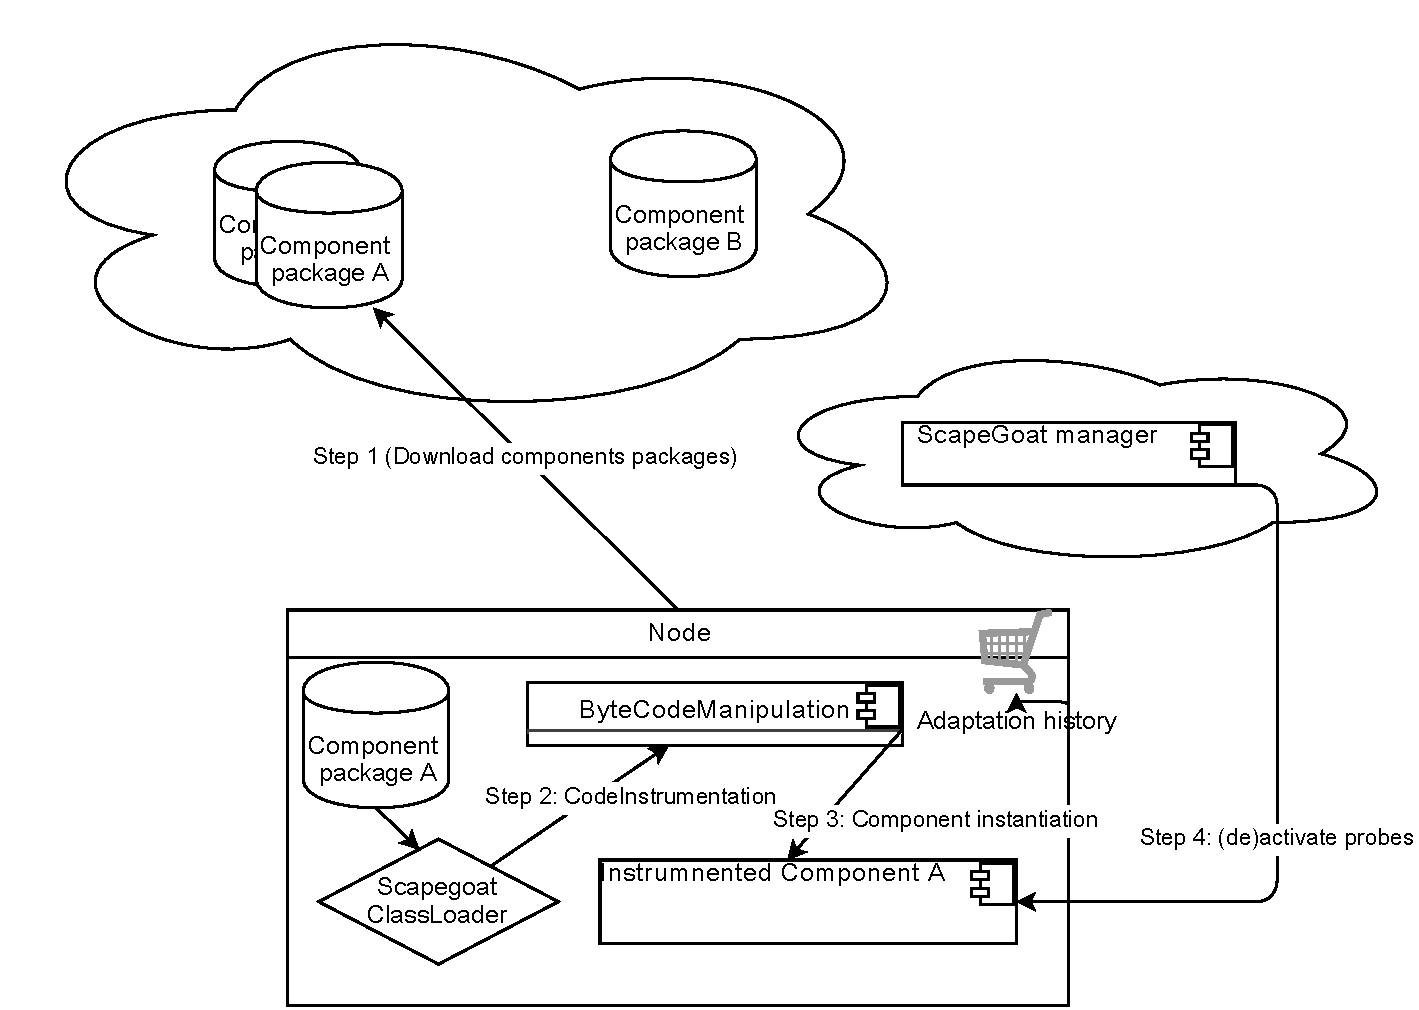
\includegraphics[scale=0.4]{figures/approach}
%	\caption{\label{fig:approach}Approach overview}
%	\end{figure}


\subsubsection{ScapeGoat's architecture}

The Scapegoat framework is built using the Kevoree component framework.
Scapegoat extends Kevoree by providing a new Node Type and three new Component Types:
\begin{itemize}
\leftskip -.2in
\item \textbf{Monitored Node.}
Handles the admission of new components by storing information about resource availability.
Before admission, it checks the security policies and registers components with a contract in the monitoring framework.
Moreover, it intercepts and wraps class loading mechanisms to record a component type's loaded classes.
Such information is used later to (de)activate the probes.
\item \textbf{Monitoring Component.}
This component type is in charge of checking component contracts. 
Basically, it implements a complex variant of the algorithm in listing \ref{algo:monitoring}.
It communicates with other components to identify suspected components.
% and to adapt the system after a fault is identified.
%todo: WHAT DOES THIS MEAN? Additionally, it makes use of another software artifact to deal with the (de)activation of probes. 
\item \textbf{Ranking Component.}
This is an abstract Component Type; therefore it is user customizable.
It is in charge of implementing the heuristic that ranks the components from the most likely to be faulty to the least likely.
\item \textbf{Adaptation component.}
This component type is in charge of dealing with the adaptation of the application when a contract violation is detected.
It is also a customizable component.
The adaptation strategy whenever a faulty component is discovered is out os scope of this paper.
Nevertheless, several strategies may be implemented in Scapegoat, such as removing faulty components or slowing down communication between components when the failure is due to a violation in the way one component is using another.
\end{itemize}

\subsubsection{Extensibility of the ScapeGoat Framework}
%\todo{For Walter: Review this section}
%\todo{We need to talk about three things: the heuristics, the admission control and the contracts semantics or implementation extensibility}

The scapegoat framework has been built with the idea of being as generic as possible, thus supporting various extensions and specializations.
In this section we discuss the extension points provided by the ScapeGoat framework.

%Defining heuristics to rank components is a part of the framework that can be specialized 
Heuristics used to rank suspected faulty components can be highly specialized
and, as we show in section~\ref{sec:evaluation}, have a remarkable impact on the behavior of ScapeGoat.
A new heuristic is created by defining a component that implements an interface to provide a ranking of the suspected components.
To do so, a context is sent with each ranking request on this component.
This context is composed of three elements, 
i) a model that describes the components and links of the deployed application, 
%ii) a models' history which contains all the models that have been deployed on the platform, and 
ii) a history that contains all the models that have been deployed on the platform, and 
iii) a history of failures composed of metadata regarding what components have failed as well as why and when it happened.
In this paper, we present three heuristics.
The first heuristic is proposed in section~\ref{sec:heuristic-based-on-modeling} and shows how we can leverage the Models@Run.time paradigm to guide the framework in finding the component that is behaving abnormally.
Due to their simplicity, the other two heuristics are presented in section~\ref{sec:evaluation} where we use them to evaluate the behavior of ScapeGoat.

The mechanism for creating new heuristics is based on the strategy design pattern. Fig~\ref{fig:strategy} illustrates this extension point. 


\begin{figure}[!h]
\centering
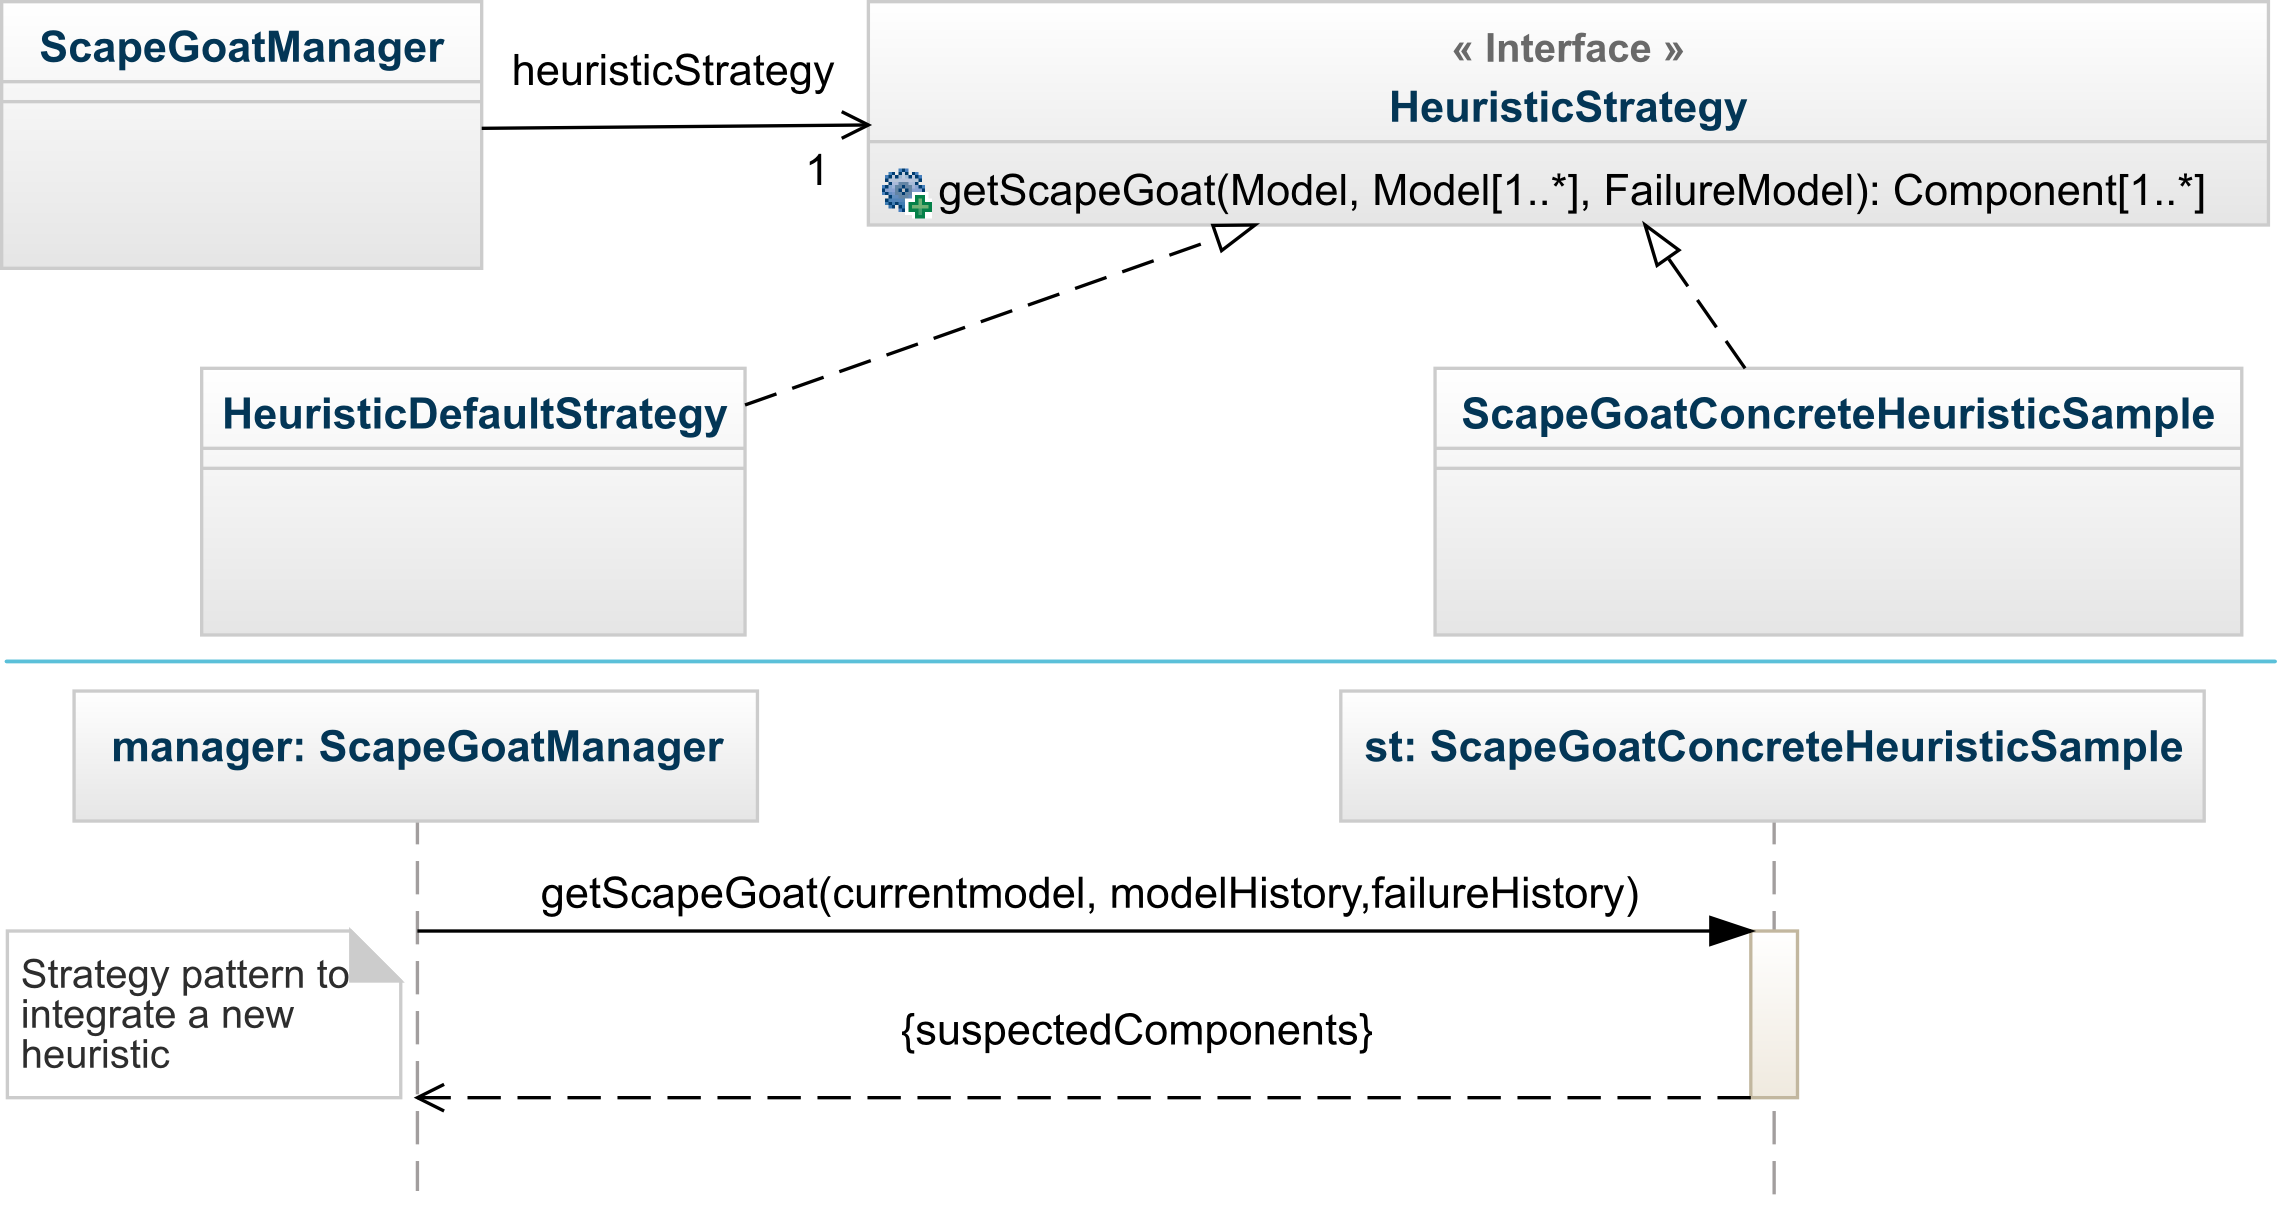
\includegraphics[width=0.9\textwidth]{./chapter5/figures/strategy}
\caption{\label{fig:strategy}Scapegoat's extensibility}
\end{figure}



A second extensible aspect of the framework is the admission control system.
The framework provides an API to hook user-defined actions when new components are submitted for deployment.
Basic data describing the execution platform in terms of resource availability, information about the already deployed components and the new component's contract are sent to the user-defined admission control system.
On each request, the admission control system has to accept or refuse the new component.
In this paper, we are using an approach which check the theoretical availability of resources whenever a component is deployed, and accept the new component if the contract can fit in the remaining available resources.
ScapeGoat is meant to support other policies as, for instance, overcommitment.
 
A last element that can be specialized to user needs is the contracts semantic.
In section~\ref{componentcontract} we describe how we interpret the contract in this work.
However, it is possible to define other contract semantics, for instance, accepting values that are closed to the limit defined in the contract, or using fuzzy values instead of sharp values.
It is worth noting that modifying the semantic of the contract would likely involved redefining the domain-specific language to describe contract and also modifying the admission control system.
 
%There are many customizable features in the framework.
%Other aspects to modify are the admission control algorithm used and the logic to check if a component behaves according its contract.
%Users of the framework can also redefine the mechanism to monitor communication among components, as we do in section~\ref{sec:WebStudy}, in order to fully capture communication based on other channels.
%Finally, in a solution that really support reconfiguration, it is essential to provide adaptation strategies.


\subsubsection{Implementation strategy}
Scapegoat aims at minimizing monitoring overhead when the framework is monitoring the global behavior of the JVM. 
To achieve this, ScapeGoat uses as few probes as possible when executing in global monitoring mode.
Only when it is necessary, ScapeGoat activates the required probes.
This features are implemented in the framework in three modules that are in charge of different concerns: a module to activate/deactivate the probes, a module to collect the resource usage, and a module to compute what components should be carefully monitored.
In this section we focus on the modules for activating/deactivating probes and for collecting information of resource usage because they required considerable engineering effort.
Notice, however, that this module is executed on demand when the framework already decides the monitoring mode to use and what components to monitor.

\paragraph{Module to activate/deactivate probes}
In ScapeGoat  we use bytecode instrumentation to perform localized monitoring.
However, instead of doing as previous approaches that manipulate the bytecode that defines components just when the component's code is executed for the first time, we modify the bytecode many times during components' life.
Every time the monitoring mode is changed we either activate or deactivate the probes by simply inserting them in the bytecode or by removing them. 
Implementing this mechanism at per-component basis requires knowing all the classes that have been loaded for a component.
This information is kept using a dictionary in which we treat a component's id as a key and a set of class names as a value.
The dictionary is filled using the \textit{traditional} classloader mechanism of Java.
In short, when a class is loaded on behalf of a component, we detect the class name and the thread that is loading the class.
Using the thread's id we are able to identify the component because we use special naming conventions for each thread executing the initial code of a component.
When probes are activated/deactivated on a component, iterating over the set of class names allows the re-instrumentation of each involved class.

The probes perform two actions: collecting data about the local usage of resources (e.g., objects recently allocated, instructions executed in the current basic block, bytes sent through the network), and notifying to the resource consumption monitor about the collected data. 
Some data we collect is computed statically when the bytecode is loaded.
This includes the size of each basic block and the size of each object allocated when the size of each instance of the class is already known.
Other data, such as bytes sent through the network or the size of allocated arrays, can only by collected dynamically when the code is running.
To notify about the collected data we use simple method calls to a proxy class in charge of forwarding the data to the monitoring module.
Probes to detect CPU consumption are inserted at the end of each basic block.
These probes collect the size in number of instructions of its container basic block.
Probes for IO throughput and network bandwidth are added in a few selected method defined in classes of the Java Development Kit (JDK).
These probes take the needed information from local variables (e.g., number of bytes) and call the proxy class. 

Our implementation, which is built using the ASM library~\footnote{asm.ow2.org} for bytecode manipulation and a Java agent to get access to and transform the classes, is based on previous approaches to deal with resource accounting and profiling in Java~\cite{binder_portable_2006,Binder200645,czajkowski_jres:_1998}.
As in previous approaches, we compute the length of each basic block to count the number of executed instructions and we try to keep a cache of \textit{known} methods with a single basic block.
Moreover, we compute the size of each object once it is allocated and we use \textit{weak} references instead of \textit{finalizers} to deal with deallocation.

\paragraph{Module to collect information regarding resource usage}
In Scapegoat, there are two mechanisms to collect information about how components consume resources.

The first mechanism is able to capture the usage of CPU, IO throughput, network bandwidth and memory.
Every time a probe that was inserted in the code of a component is executed, the proxy class forwards the local resource usage to the module in charge of collecting the resource usage.
Along with the local resource usage, probes also notify the id of the components consuming resource.
Such data is then used to aggregate the global consumption of each component.
It is worth noting that, when this first mechanism is used to collect memory consumption, on object is always accounted as  consumed for the component responsible for its initial allocation.
In short, no matter whether the initial component $C$ that allocates the object no longer held a reference to an object $O$, as long as $O$ remains in memory, $C$ is accounted for its consumption.
Moreover, as was already mentioned, using this mechanism is not possible to deactivate the probes related to memory consumption.

On the contrary, the second mechanism is only useful to collect information about memory consumption.
The advantages of this method are: we can leverage the proposed optimistic monitoring because it executes only on demand, and it has no impact on the number of objects allocated in memory because no \textit{weak references} are used.
However, in this method an object $O$ is consumed not for the component that allocates it but for those components that held references to it.
As a consequence, in certain occasions the framework states that an object is being consumed for many components at the same time. 
We built this solution on top of the JVM Tool Interface (JVMTI) by implementing the algorithm proposed in~\cite{Price:2003:GCM:829515.830545, Geoffray5270296}, with the main difference being that our solution works without modifying the garbage collector.
In summary, this algorithm simply try to find those objects that are reachable from the references of each component.
It does so by traversing the graph of live object using as the component instance and its threads as roots of the traversal. 
Since our approach does not require a modification to the garbage collector, it is portable and works with different garbage collector implementations.

%\subsubsection{Quality of Contract} 

%\todo{}
%\todo{do not forget to have a part on implementation}

\subsection{Leveraging Models@run.time to build an efficient monitoring framework}\label{sec:heuristic-based-on-modeling}
As presented in section \ref{monitorContainer}, our approach offers a dynamic way to activate and deactivate fine-grain localized monitoring.
We use a heuristic to determine which components are more likely to be faulty.
Suspected components are the first to be monitored.

%\hl{Isn't this a conclusion of the evaluation? Why is it here?}
%When compared to fine-grain monitoring of all components, our technique decreases the accumulated overhead of the monitoring system when a problem is detected.
%It should be noted that a poorly performing heuristic may introduce extensive delays in identifying faulty components.
%With this in mind, our approach is a trade-off between low monitoring overhead and the delay introduced to identify the faulty component (i.e., overhead versus latency).
%Thus, the overall performance of our approach is tightly coupled to the performance of our heuristic in accurately finding faulty components.

Our framework can support different heuristics, which can be application or domain-specific.
In this paper we propose a heuristic that leverages the use of the Models@run.time approach to infer the faulty components.
The heuristic is based on the assumption that the cause of newly detected misbehavior in an application is likely to come from the most recent changes in the application.
This can be better understood as follows:
\begin{itemize}
\leftskip -.2in
  \item recently added or updated components are more likely to be the source of a faulty behaviour;
  \item components that directly interact with recently added or updated components are also suspected.
\end{itemize}

We argue that when a problem is detected it is probable that recent changes have led to this problem, or else, it would have likely occurred earlier.
If recently changed components are monitored and determined to be healthy, it is probable that the problem comes from direct interactions with those components.
Indeed, changes to interactions can reveal dormant issues with the components.
The algorithm used for ranking the components is presented in more detail in listing \ref{algo:heuristic}.
%todo: WHAT???? Note that in this heuristic, each subset of components to be finely monitored is composed for one element of the list.
In practice, we leverage the architectural-based history of evolutions of the application, which is provided by the Models@run.time approach.
%The heuristic starts at the most recently changed components, because they are more likely to have introduced the problem, and we iteratively move to older components.


\begin{lstlisting}[escapeinside={(*}{*)},caption=The ranking algorithm (uses the model history for ranking).,label=algo:heuristic,float=!h]
ranker() : list<Component>
	// used to avoid adding duplicated elements to the list
	visited = (*$\emptyset$*)
	// this list will contain the result of calling the routine
	ranking = {}
	for each model M (*$\in$*) History
		// adding components that were added in this model
		N = {c (*$\mid$*) c was added in M}
		ranking.add N(*$\setminus$*)visited
		visited = visited (*$\cup$*) N
		// finding neighbors
		Neighbors (*$ = \bigcup_{c \in N}{c.neighbors}$*)
		SortedNeighbors = sort (Neighbors (*$\setminus$*) visited, History)
		// adding neighbors
		ranking.add SortedNeighbors
		visited = visited (*$\cup$*) Neighbors
	// return the built ranking
	return ranking

// this routine recursively sort a set of components using the following criteria:
// components are sorted by the timestamp that indicates when they were installed
private sort (S : Set<Component>, H : History) : list<Component>
	r = {}
	if (*$S \ne \emptyset$*)
		choose (*$b \mid b \in S$*) (*$\wedge$*) b is newer with respect to H than any other element in S
		r.add b, sort (S(*$\setminus$*){b}, H)
	return r
\end{lstlisting}

Listing~\ref{algo:heuristic} shows two routines, but only routine \textit{ranker} is public.
It can be called by the monitoring system when it is necessary to figure out in what order components must be carefully monitored. 
After initializing an empty list which will hold the rank, the algorithm starts to iterate in line 4 over the history of models that have been installed in the system.
As mentioned, this history contains a sorted set of models that describe what components have been installed in the system.
Within each iteration, the algorithm first computes in line 5 the set of components that were installed at such a point in time.
Afterwards, these components are added to the result.
The next step, executed at lines 8 and 9, is finding those components that are directly connected to components that were added to the application at this point in time.
Finally, these \textit{neighbors} are added to the rank after being sorted.
Routine \textit{sort} simply sorts a set of components using as criteria the time at which components where installed in the system.

%We implemented this alogrithm using the kevoree framework that provide the model to know the interactions between components and which offer access to the model history.
%\subsection{Analysis of expected behaviour}\label{analysis}
%
During adaptive monitoring, the monitoring system transits between either \textit{Global} lightweight monitoring (G) and \textit{All Components} or full monitoring (F), or Global and \textit{Specific} monitoring based on heuristics (H).
We can describe the transitions back and forth as:
\begin{subequations}
\begin{align}
G \rightarrow F \label{tA1}
\\F \rightarrow G \label{tA2}
\end{align}
\end{subequations}
\begin{subequations}
\begin{align}
G \rightarrow H \label{tH1}
\\ H \rightarrow G \label{tH2}
\end{align}
\end{subequations}
Different monitoring modes have different times to detect a failure.
We denote by $T_{df}(F),T_{df}(G),T_{df}(M_x)$ the time to detect failure of full, global and subset monitoring respectively. 
We know by construction that relations \eqref{dt0}, \eqref{dt1} and \eqref{dt2} hold.
This means that full monitoring should detect both the existence of a fault and the source of a fault faster than adaptive monitoring because all components are continuously checked instead of just a lightweight global check\footnote{It should be noted that the lightweight global monitoring mode can only detect the existence of a fault but not the source of the fault. To detect the source of the fault, more intrusive, per-component monitoring is required}.
However, there is no direct relationship between the two variants of adaptive monitoring (i.e., \eqref{dt1} and \eqref{dt2}) because the delay depends on the time needed to probe and instrument components (varies according to the number and size of classes), and the quality of the heuristic in targeting faulty components as quickly as possible.
The former element affects the delay when \textit{all components} are instrumented.
The latter depends on the ability of the heuristic to include the faulty component inside the set of suspected faulty components.
\begin{subequations}
\begin{align}
T_{df}(F) \le T_{df}(G) \label{dt0}
\\ T_{df}(F) \le T_{df}(G) + \sum_{i=0}^{j}(T_{trans}(C_i) + T_{df}(M_i)) \label{dt1}
\\ T_{df}(F) \le T_{df}(G) + T_{trans}(all) + T_{df}(M_{all}) \label{dt2}
\end{align}
\end{subequations}
%The experiments have shown the impact of monitoring policies over performance.
Another important dimension is the global overhead of each policy on the running system.
The following relations apply to this dimension.
Relation \eqref{overheadRelations1} is true because Full monitoring is always costlier than lightweight Global monitoring.
Relations \eqref{overheadRelations2} and \eqref{overheadRelations3} are true if a single faulty behaviour occurs during the execution of the application.
However, these relations do not apply when the number of failures and the number of transitions grow.
It is also impossible to establish a relation between the two adaptive monitoring policies because, once again, it depends on the size of the application and the quality of the heuristic in quickly finding the source of faults. 
\begin{subequations}
\begin{align} 
 O(F) > O(G) \label{overheadRelations1}
\\ O(F) > O(G) + O_{trans}(all) + O(M_{all}) \label{overheadRelations2}
\\ O(F) > O(G) + \sum_{i=0}^{j}(O_{trans}(C_i) + O(M_i)) \label{overheadRelations3}
\end{align}
\end{subequations}
Only relationship \eqref{overheadRelations1} is independent of the application.
The other relationships depend on time.
We can express overhead as a time dependent function.
For instance, let $O_F(t)$,  $O_A(t)$ be the overhead in the application due to Full monitoring and Adaptive monitoring with all components respectively.
Where: 
\begin{equation*}
O_F(t)\approx const
\end{equation*}
\begin{equation*} 
O_A(t) = 
	\begin{cases}
   		O(G) & \text{if in G state} \\
   		O_{trans}(all) & \text{if changing state in t} \\
   		O(M_{all})=O(F) & \text{if in A state}
  	\end{cases} 
\end{equation*}
The integral expresses the overhead in a given amount of time.
The relation \eqref{eq:overhead-time} is true under two conditions.
On the one hand, if time spent in global monitoring is bigger than time spent in other states.
On the other hand, if the overhead due to transitions is small.
A similar analysis is applicable to adaptive monitoring based on heuristics.
\begin{equation}
\int O_F(t)\,dt > \int O_A(t)\,dt \label{eq:overhead-time}
\end{equation}
The first condition is reasonably met through the two following factors.
First, we can expect that most applications have few failures in comparison to the global execution time of the application.
Second, the application container should provide an adaptation mechanism to remove the source of failure when a contract violation is identified.
This adaptation would allow the system to transition back into global monitoring.

Following the previous analysis we can conclude that the overhead of the monitoring framework depends on the following factors: the time spent in global monitoring, the number of transitions performed to intrusive monitoring, the quality of the heuristic, and the size of the application.
Likewise, the quality of the heuristic and the size of the application affect the delay to detect failures.
%We can now see that the behavior of \textit{all monitoring} strategy is due to the hostile execution environment we are using.
%The behavior change completely if we introduce an adaptation mechanism to remove the faulty component instead of allowing the its uncontrolled execution.


